\documentclass[tikz,border=3.14mm]{book}
\usepackage{amsmath,amssymb}
\usepackage{tikz}
\usetikzlibrary{tikzmark, calc}
\begin{document}
    \vspace{4ex}
    {\Large
    \begin{equation*}
        \tikzmark{sum}\sum_{\tikzmark{ind}i=\tikzmark{un}1}^{\tikzmark{up}n} = {a}_{i}\tikzmark{elem}
    \end{equation*}}
    \begin{tikzpicture}[overlay,remember picture]
        \draw ($(pic cs:sum)+(.1,.15)$) --  ($(pic cs:sum)+(-.85,.15)$) 
            node[anchor=east] 
                {\footnotesize summation sign};
        \draw ($(pic cs:ind)+(.07,-.08)$) |- ($(pic cs:ind)+(-1,-.3)$) 
            node[anchor=east,text width=3cm] 
                {\vspace{-1ex}
                 \begin{flushright} 
                     \footnotesize 
                     index of \\ 
                     summation 
                 \end{flushright}};
        \draw ($(pic cs:up)+(.09,.25)$) |- ($(pic cs:upb)+(6.6,2.1)$) 
            node[text width=7cm, anchor=west] 
                {\vspace{-1ex}
                 \begin{flushleft} 
                     \footnotesize 
                     stopping point \\ 
                     upper limit of summation 
                 \end{flushleft}};
        \draw ($(pic cs:elem)+(.1,.15)$) -- ($(pic cs:elem)+(.9,.15)$) 
            node[anchor=west, text width=3cm] 
                {\footnotesize typical element};
        \draw ($(pic cs:un)+(.09,-.08)$) |- ($(pic cs:un)+(1,-.3)$) 
            node[anchor=west, text width=7cm] 
                {\vspace{-1ex}
                 \begin{flushleft} 
                     \footnotesize 
                     starting point\\ 
                     lower point of summation 
                 \end{flushleft}};
    \end{tikzpicture}

    \vspace{7mm}
\end{document}